\documentclass[journal,12pt,twocolumn]{IEEEtran}

\usepackage{setspace}
\usepackage{gensymb}

\singlespacing


\usepackage[cmex10]{amsmath}

\usepackage{amsthm}

\usepackage{mathrsfs}
\usepackage{txfonts}
\usepackage{stfloats}
\usepackage{bm}
\usepackage{cite}
\usepackage{cases}
\usepackage{subfig}

\usepackage{longtable}
\usepackage{multirow}

\usepackage{enumitem}
\usepackage{mathtools}
\usepackage{steinmetz}
\usepackage{tikz}
\usepackage{circuitikz}
\usepackage{verbatim}
\usepackage{tfrupee}
\usepackage[breaklinks=true]{hyperref}
\usepackage{graphicx}
\usepackage{tkz-euclide}

\usetikzlibrary{calc,math}
\usepackage{listings}
    \usepackage{color}                                            %%
    \usepackage{array}                                            %%
    \usepackage{longtable}                                        %%
    \usepackage{calc}                                             %%
    \usepackage{multirow}                                         %%
    \usepackage{hhline}                                           %%
    \usepackage{ifthen}                                           %%
    \usepackage{lscape}     
\usepackage{multicol}
\usepackage{chngcntr}

\DeclareMathOperator*{\Res}{Res}

\renewcommand\thesection{\arabic{section}}
\renewcommand\thesubsection{\thesection.\arabic{subsection}}
\renewcommand\thesubsubsection{\thesubsection.\arabic{subsubsection}}

\renewcommand\thesectiondis{\arabic{section}}
\renewcommand\thesubsectiondis{\thesectiondis.\arabic{subsection}}
\renewcommand\thesubsubsectiondis{\thesubsectiondis.\arabic{subsubsection}}


\hyphenation{op-tical net-works semi-conduc-tor}
\def\inputGnumericTable{}                                 %%

\lstset{
%language=C,
frame=single, 
breaklines=true,
columns=fullflexible
}
\begin{document}


\newtheorem{theorem}{Theorem}[section]
\newtheorem{problem}{Problem}
\newtheorem{proposition}{Proposition}[section]
\newtheorem{lemma}{Lemma}[section]
\newtheorem{corollary}[theorem]{Corollary}
\newtheorem{example}{Example}[section]
\newtheorem{definition}[problem]{Definition}

\newcommand{\BEQA}{\begin{eqnarray}}
\newcommand{\EEQA}{\end{eqnarray}}
\newcommand{\define}{\stackrel{\triangle}{=}}
\bibliographystyle{IEEEtran}
\providecommand{\mbf}{\mathbf}
\providecommand{\pr}[1]{\ensuremath{\Pr\left(#1\right)}}
\providecommand{\qfunc}[1]{\ensuremath{Q\left(#1\right)}}
\providecommand{\sbrak}[1]{\ensuremath{{}\left[#1\right]}}
\providecommand{\lsbrak}[1]{\ensuremath{{}\left[#1\right.}}
\providecommand{\rsbrak}[1]{\ensuremath{{}\left.#1\right]}}
\providecommand{\brak}[1]{\ensuremath{\left(#1\right)}}
\providecommand{\lbrak}[1]{\ensuremath{\left(#1\right.}}
\providecommand{\rbrak}[1]{\ensuremath{\left.#1\right)}}
\providecommand{\cbrak}[1]{\ensuremath{\left\{#1\right\}}}
\providecommand{\lcbrak}[1]{\ensuremath{\left\{#1\right.}}
\providecommand{\rcbrak}[1]{\ensuremath{\left.#1\right\}}}
\theoremstyle{remark}
\newtheorem{rem}{Remark}
\newcommand{\sgn}{\mathop{\mathrm{sgn}}}
\providecommand{\abs}[1]{\left\vert#1\right\vert}
\providecommand{\res}[1]{\Res\displaylimits_{#1}} 
\providecommand{\norm}[1]{\left\lVert#1\right\rVert}
%\providecommand{\norm}[1]{\lVert#1\rVert}
\providecommand{\mtx}[1]{\mathbf{#1}}
\providecommand{\mean}[1]{E\left[ #1 \right]}
\providecommand{\fourier}{\overset{\mathcal{F}}{ \rightleftharpoons}}
%\providecommand{\hilbert}{\overset{\mathcal{H}}{ \rightleftharpoons}}
\providecommand{\system}{\overset{\mathcal{H}}{ \longleftrightarrow}}
	%\newcommand{\solution}[2]{\textbf{Solution:}{#1}}
\newcommand{\solution}{\noindent \textbf{Solution: }}
\newcommand{\cosec}{\,\text{cosec}\,}
\providecommand{\dec}[2]{\ensuremath{\overset{#1}{\underset{#2}{\gtrless}}}}
\newcommand{\myvec}[1]{\ensuremath{\begin{pmatrix}#1\end{pmatrix}}}
\newcommand{\mydet}[1]{\ensuremath{\begin{vmatrix}#1\end{vmatrix}}}
\numberwithin{equation}{subsection}
\makeatletter
\@addtoreset{figure}{problem}
\makeatother
\let\StandardTheFigure\thefigure
\let\vec\mathbf
\renewcommand{\thefigure}{\theproblem}
\def\putbox#1#2#3{\makebox[0in][l]{\makebox[#1][l]{}\raisebox{\baselineskip}[0in][0in]{\raisebox{#2}[0in][0in]{#3}}}}
     \def\rightbox#1{\makebox[0in][r]{#1}}
     \def\centbox#1{\makebox[0in]{#1}}
     \def\topbox#1{\raisebox{-\baselineskip}[0in][0in]{#1}}
     \def\midbox#1{\raisebox{-0.5\baselineskip}[0in][0in]{#1}}
\vspace{3cm}
\title{Assignment-6}
\author{Ankur Aditya - EE20RESCH11010}
\maketitle
\newpage
\bigskip
\renewcommand{\thefigure}{\theenumi}
\renewcommand{\thetable}{\theenumi}

\begin{abstract}
This document contains the procedure to find the equation of tangent to parabola.
\end{abstract}
Download the python code from 
\begin{lstlisting}
https://github.com/ankuraditya13/EE5609-Assignment6
\end{lstlisting}
%
and latex-file codes from 
%
\begin{lstlisting}
https://github.com/ankuraditya13/EE5609-Assignment6
\end{lstlisting}

\section{Problem}
Find the equation of the tangent to the curve,
\begin{align}
y = \sqrt{3x-2}
\label{Q}
\end{align}
 which is parallel to the line,
\begin{align}
\myvec{4&2}\vec{x}+5=0
\label{P}
\end{align}  
\section{Solution}
The equation \eqref{Q} can be written as,
\begin{align}
y^2-3x+2 = 0
\end{align}
Comparing it with standard equation,
\begin{align}
ax^2+2bxy+cy^2+2dx+2ey+f = 0
\end{align}
$\therefore$ a = b = e = 0, d = $\frac{-3}{2}$, c = 1, f = 2.
\begin{align}
\therefore \vec{V} = \myvec{a&b\\b&c} = \myvec{0&0\\0&1}
\end{align} 
\begin{align}
\therefore\vec{u} = \myvec{d\\e} = \myvec{\frac{-3}{2}\\0}\label{u}
\end{align}
\begin{align}
 \mbox{ Now,} \mydet{V} = \mydet{0&0\\0&1} = 0
\end{align}
$\implies$ that the curve is a parabola. Now, finding the eigen values corresponding to the $\vec{V}$,
\begin{align}
\mydet{\vec{V}-\lambda\vec{I}} = 0
\end{align}
\begin{align}
\mydet{-\lambda&0\\0&1-\lambda} = 0
\end{align}
\begin{align}
\implies \lambda = 0,1.
\end{align}
Calculating the eigenvectors corresponding to $\lambda = 0,1$ respectively,
\begin{align}
\vec{V}\vec{x} = \lambda\vec{x}
\end{align}
\begin{align}
\myvec{0&0\\0&1}\vec{x} = 0 \implies \vec{p_1} = \myvec{1\\0}
\end{align}
\begin{align}
\myvec{0&0\\0&1}\vec{x} = \vec{x} \implies \vec{p_2} = \myvec{0\\1}
\end{align}
Now by eigen decomposition on $\vec{V}$,
\begin{align}
\vec{V} = \vec{PDP^T}
\label{V}
\end{align}
\begin{align}
\mbox{where,} \vec{P} = \myvec{\vec{p_1} \vec{p_2}} = \myvec{1&0\\0&1}
\end{align}
\begin{align}
\vec{D} = \myvec{\lambda_1&0\\0&\lambda_2} = \myvec{0&0\\0&1}
\end{align}
Hence equation \eqref{V} becomes,
\begin{align}
\vec{V} = \myvec{1&0\\0&1}\myvec{0&0\\0&1}\myvec{1&0\\0&1}
\end{align}
\begin{align}
\vec{V} = \myvec{0&0\\0&1}
\end{align}
Now the tangent to parabola is parallel to the line equation \eqref{P}, Hence the direction vectors ($\vec{m}$) and normal ($\vec{n}$)  vectors are,
\begin{align}
\vec{m} = \myvec{1\\-2}\\
\vec{n} = \myvec{2\\1}\label{n}
\end{align} 
Now, the equation for the point of contact for the parabola is given as,
\begin{align}
\myvec{\vec{u}^T+\kappa\vec{n}^T\\\vec{V}}\vec{q} = \myvec{-f\\\kappa\vec{n}-\vec{u}}\label{contact}\\
\mbox{where, } \kappa = \frac{\vec{p_1}^T\vec{u}}{\vec{p_1}^T\vec{n}} = \frac{-3}{4} \label{k}
\end{align}
Hence substituting the values of \eqref{k}, \eqref{n}, \eqref{V} and \eqref{u} in equation \eqref{contact} we get,
\begin{align}
\myvec{-3&\frac{-3}{4}\\0&0\\0&1}\vec{q} = \myvec{-2\\0\\\frac{-3}{4}}
\label{solve_q}
\end{align}
Solving for $\vec{q}$ by removing the zero row and representing \eqref{solve_q} as augmented matrix and then converting the matrix to echelon form,
\begin{align}
\implies \myvec{-3&\frac{-3}{4}&-2\\0&1&\frac{-3}{4}} \xleftrightarrow[]{R_1\leftarrow\brak{\frac{-R_1}{3}}} \myvec{1&\frac{1}{4}&\frac{2}{3}\\0&1&\frac{-3}{4}}
\end{align}
\begin{align}
\xleftrightarrow[]{R_1\leftarrow R_1-\frac{1}{4}R_2} \myvec{1&0&\frac{41}{48}\\0&1&\frac{-3}{4}}
\label{q_value}
\end{align}
Hence from equation \eqref{q_value} it can be concluded that the point of contact is,
\begin{align}
\vec{q} = \myvec{\frac{41}{48}\\\frac{-3}{4}}
\end{align}
Now $\vec{q}$ is a point on the tangent. Hence, the equation of the
line can be expressed as
\begin{align}
\vec{n}^T\vec{x} = c
\label{tangent}
\end{align}
where c is,
\begin{align}
 c = \vec{n}^T\vec{q} = \myvec{2&1}\myvec{\frac{41}{48}\\\frac{-3}{4}} = \frac{23}{24} 
 \label{const}
\end{align}
Hence equation of tangent to the curve \eqref{Q} parallel to \eqref{P} is given by substituting the value of c and $\vec{n}$ from equation \eqref{const} and \eqref{n} respectively to the equation \eqref{tangent},
\begin{align}
\implies\myvec{2&1}\vec{x} = \frac{23}{24} 
\end{align}
Figure \ref{Figure_1} verifies that the $\myvec{2&1}\vec{x} = \frac{23}{24}$ is a tangent to parabola  $y=\sqrt{3x-2}$
\begin{figure}[ht!]
\centering
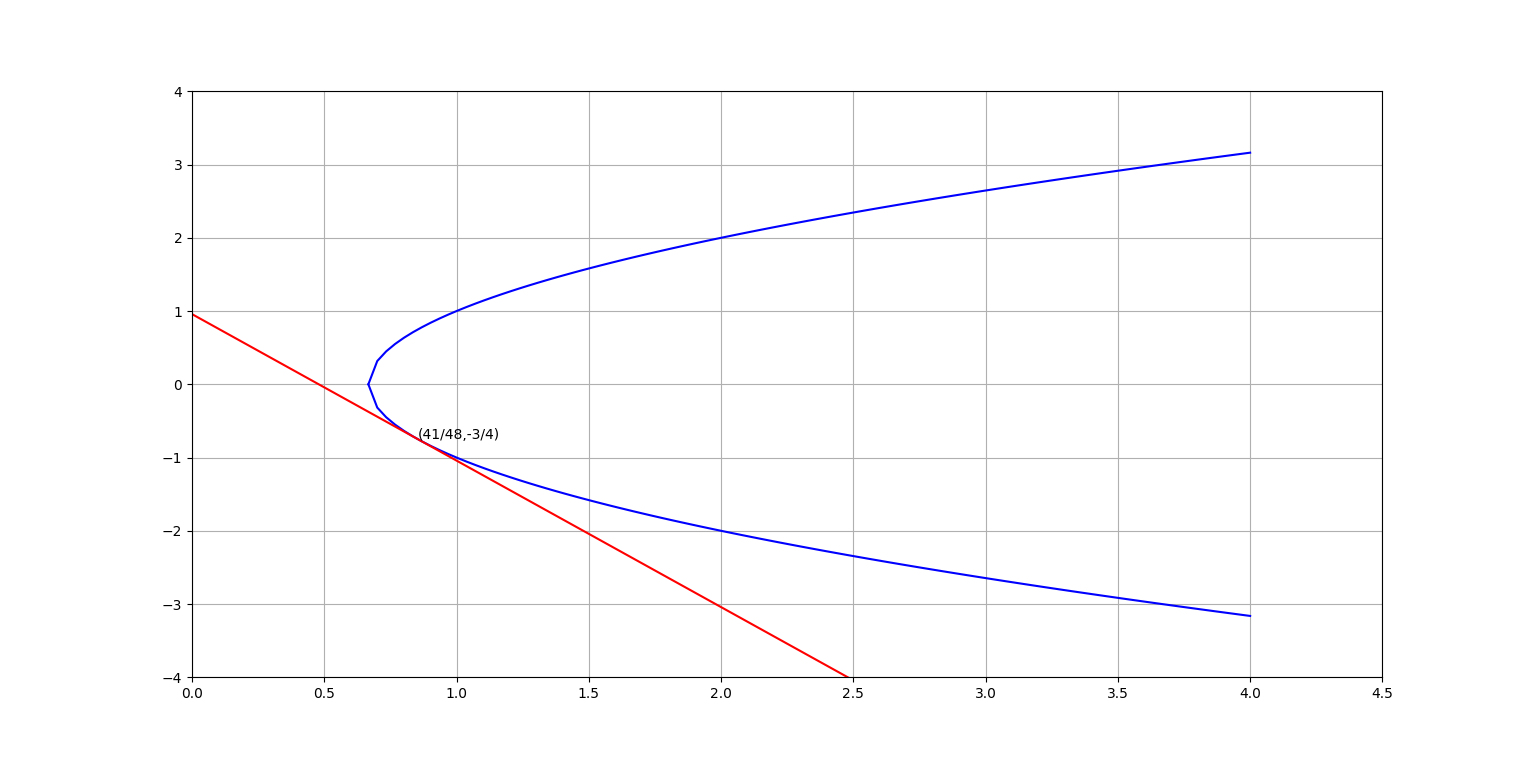
\includegraphics[width=\columnwidth]{Figure_1.png}
\caption{Tangent to parabola $y=\sqrt{3x-2}$}
\label{Figure_1}
\end{figure}
\end{document}
